\documentclass[letter]{article}

\usepackage{amsmath}
\usepackage{graphicx}
\usepackage{geometry}
\usepackage{braket} %Can do bra-ket notation with \braket{}
\usepackage{framed} %Adds the framed environment
\usepackage{fancyhdr}
\usepackage{datetime} %For formatting of header date
\usepackage{ulem} %Makes strike-through lines with \sout{}
\usepackage{booktabs} %better tables
\usepackage{multirow} %Support multi-row in tables
\usepackage[table,xcdraw]{xcolor} %Support colored rows in tables
\usdate %Month, Dth, YYYY
\geometry{
  letterpaper,
  left=1in,
  right=1in,
  bottom=1in,
  top=1in}
\pagestyle{fancy}
\lhead{NE101 Final Study Guide}
\chead{}
\rhead{}
\lfoot{}
\cfoot{\thepage}
\rfoot{\today \quad \currenttime}
\setlength\parindent{0pt}

\begin{document}
\textbf{\Large{Nuclear Engineering 101: Final Study Guide}} \\
\vspace{12pt}
%\cite[pp. 45]{krane}
%\cite[Lec 24]{lecture}

\textbf{Disclaimer:} This is not an official study guide. Stuff \sout{might}
\textbf{is} wrong. Use the lecture notes and book!
\vspace{10pt}

\textbf{Note:} Everything in this guide is from the text (Krane) or
lecture, or office hours and should be cited as completely as
possible.

\tableofcontents

\section{Reactions}

\subsection{General Information}

\begin{itemize}
\item The reaction:
  \begin{equation*}
    a + X \to Y + b
  \end{equation*}
Can be written in reaction notation as:
\begin{equation*}
  X(a,b)Y
\end{equation*}
\cite[pp. 378-379]{krane}
\item A microscopic cross section ($\sigma$) represents the ``relative
  probability for the reaction to occur.'' It can be used in the
  following equation:
  \begin{equation*}
    \begin{split}
      R= (\rho{}d)_{target}\times{}I_{beam}\times\sigma_{reaction}
    \end{split}
  \end{equation*}
Where $R$ is the reaction rate (in reactions/sec/cm$^2$); $(\rho{}d)$ is the
density (in g/cm$^3$) times the width of the target (in cm), also
known as the areal density (this needs to be converted to atoms/$cm^2$); $I_{beam}$ is the incident particle flux
(in atoms/sec/cm$^2$); and $\sigma_{reaction}$ is the microscopic cross
section of the reaction occurring. This is only valid when very little
of the beam reacts (small $\sigma$) and everything moves in straight
lines. Note that is it common practice to drop the 1/cm$^2$ from the
reaction rate and beam current ($I$) by assuming that the target is
exactly 1 cm$^2$ in size. This can also be formulated as:
\begin{equation*}
  R = NdI_{beam}\sigma_{reaction}
\end{equation*}
In this case, $N$ is explicitly the number density of the target
material (in atoms/cm$^3$) and $d$ is the width of the target (in
cm). This is exactly equivalent to the last equation, but $\rho{}d$
has been converted into number density.

\vspace{10pt}
It can also be expressed in terms of flux as:
\begin{equation*}
        R= n\phi\sigma
\end{equation*}
Where $n$ is the number density of target atoms (in atoms/cm$^3$), $\phi$ is the flux in
(atoms/sec/$cm^2$) and $\sigma$ is the same. This will give a reaction
rate in units of reactions/$cm^3$.~\cite[Lec. 25]{lecture}
\begin{framed}
  \textbf{Current vs. Flux:} In general, the incident beam current $I$
  is used when you have a beam of particles on a target, hence it is
  formulated with the number density of the target and the width of
  the target. This is also why the reaction rate is reactions/sec/area
  of the target. Flux is generally used when you have a bunch of
  particles \textit{inside} a material causing reactions. Then you are
  more interested in the number density of the material, and your
  reaction rate is in reactions/sec/unit volume.

  In the end, it doesn't really matter if you get the units
  right. Dimensional analysis will save you.
\end{framed}
\item Microscopic cross sections are generally given in units of
  barns. 1 barn = $10^{-24}$ cm$^2$.
  \item The cross section is not always constant over angle (it rarely
    is). So the \textit{differential cross section} is used:
    \begin{equation*}
      \frac{d\sigma}{d\Omega}
    \end{equation*}
    What is confusing, is this is just
    a number, in units of barns/steradian. It's
    representing the fact that some small number of particles
    ($d\sigma$) will strike our small detector ($d\Omega$). It is
    dependent on the angle of scatter ($\theta$) and the polraization
    of the radiation ($\phi$). Generally we assume there is no affect
    due to polarization (things are randomly polarized).

We can
    find the size of our detector $d\Omega$ in steradians, which is
    related to the area of our detector ($dA$) and the distance from
    the target ($r$) by:
    \begin{equation*}
      d\Omega = \frac{dA}{r^2}
    \end{equation*}
    Then, if we know the differential cross section at the angle of
    our detector, we can multiply to get the reaction cross section
    for our detector:
    \begin{equation*}
      \sigma_{det} = d\Omega\frac{d\sigma}{d\Omega}
    \end{equation*}
    This represents something \textbf{very specific}. This is the
    probability that incoming particles striking the target will then
    be detected by our detector. Based on the size of our detector
    ($d\Omega$) and our a priori knowledge of the number of particles
    that will be seen in a small area ($\frac{d\sigma}{d\Omega}$). The
    value of that differential cross section will probably vary with
    angle, so you have to know the differential cross section for the
    angle where your detector is to even use this. More rigorously,
    you'd integrate over the area of the detector and
    $\frac{d\sigma}{d\Omega}$ may vary over the integral:
    \begin{equation*}
      \sigma_{det} = \int_{detector}\frac{d\sigma}{d\Omega}d\Omega
    \end{equation*}
    Or, you can get the total $\sigma$ by integrating over the whole
    angle space.
\item Conserved quantities in reactions:
  \begin{itemize}
  \item Total energy
  \item Linear momentum
  \item Angular momentum
  \item Parity $(-1)^l$ (except in weak interactions)
\end{itemize}
\item \textbf{Kinematics} For a reaction, $X(a,b)Y$:
  \begin{equation*}
    \begin{split}
      Q&= (m_{X}+m_{a}-m_{Y}-m_{b})c^{2}\\
      Q& =T_{Y}+T_{b}-T_{X}-T_{a}
\end{split}
\end{equation*}
\item Exothermic Q$>$0 :
  \begin{equation*}
  \begin{split}
   m_{X}+m_{a}&>m_{Y}+m_{b}\\
   T_{Y}+T_{b}&>T_{X}+T_{a}
  \end{split}
\end{equation*}
\item Endothermic Q$<$0 :
  \begin{equation*}
  \begin{split}
    m_{X}+m_{a}<&m_{Y}+m_{b}\\
T_{Y}+T_{b}<&T_{X}+T_{a}
  \end{split}
\end{equation*}
\item Reaction reaches excited states of Y:
  \begin{equation*}
Q_{ex} = (m_{X}+m_{a}-m_{Y*}-m_{b})c^{2}  = Q_{0}-E_{ex}
\end{equation*}
\item Compound nucleus:
  \begin{equation*}
Q = -T_{a} = (m_{X}+m_{a}-m_{C*})c^{2}-E_{ex}
\end{equation*}

\end{itemize}

\subsection{Photo-nuclear Interactions}

\begin{itemize}
\item A photon interacts with the nucleus directly. For this to
  happen, we need to have an energy level at the energy of the
  incoming photon.~\cite[Lec 25]{lecture}
\item There are three types of photo-nuclear interactions:
  \begin{itemize}
  \item Spontaneous emission: if the nucleus is in an energy level, it
    can release a photon to de-excite. This is an intrinsic property
    of the level.
  \item Resonant absorption: if the incoming photon is at the exact same energy
    of an energy level, it can be absorbed and the nucleus excited to
    that state. The energy of the state is the resonance energy.
  \item Stimulated emission: One photon goes in, two photons come
    out. This occurs if the incoming photon is at the resonant
    value. This is the principle by which lasers work (on the atomic
    scale), but it has not been seen for nuclei.
  \end{itemize}
  \cite[Lec 25]{lecture}
\item The cross section for this to occur ($\sigma_0$) is a function
  of the nucleus' angular momentum, and internal conversion (IC)
  factors ($\alpha$). As the probability of IC rises, photon capture
  becomes more rare, it's hard to make a nucleus capture photons when
  it wants to eject electrons.~\cite[Lec 25]{lecture}
\item The width of the emitted state:
  \begin{equation*}
    \Gamma = \frac{\hbar}{\tau}
  \end{equation*}
The longer the mean lifetime ($\tau$), the more well defined the
energy level's value is.~\cite[Lec 25]{lecture}
\end{itemize}
\subsubsection{Resonance Absorption}
\begin{itemize}
\item The resonance energy can be affected by any recoil that will
  result from the capture. This is because the nucleus needs both
  enough energy to be in its new excited state, \textbf{and} enough energy
  to recoil; so the incoming photon needs to have a little bit more
  than the expected resonance energy. As shown in
  Figure~\ref{fig:resonance_recoil}, the resonance energy has been
  shifted up by the recoil energy $E_R$ from the expected value
  $\Delta{}E$.~\cite[Lec 25]{lecture}

  \begin{figure}[hbtp]
    \centering
    \includegraphics[scale=1.0]{images/resonance_recoil}
    \caption{The resonance absorption peak is normally at $\Delta{}E$, it is
      shifted \textit{up} by the recoil energy $E_R$, Krane figure 10.23.~\cite{krane}.\label{fig:resonance_recoil}}
  \end{figure}
\item This has an exactly opposite effect on the emission
  spectrum. The absorption spectrum was shifted \textit{up} because the
  incoming photon needed extra energy to recoil the nucleus. The
  emission spectrum is shifted \textit{down} because the recoil takes some of
  the energy of the emitting photon.~\cite[Lec. 25]{lecture}
\item\textbf{Doppler broadening:} thermal motion makes the nuclei move back
  and forth, so the incoming photons energy looks doppler shifted
  either higher or lower. Therefore, a photon with energy just off the
  resonance may actually be absorbed because the relative motion can
  shift its energy to the resonance value. A wider energy range can
  now be absorbed by the resonance, so the peak gets wider or
  \textit{broadens}.~\cite[pp. 363]{krane}
\item Doppler broadening can can cause overlap between
  the emission and absorption peaks. ~\cite[Lec. 25]{lecture}
\item\textbf{Mossbauer Effect:} If a nuclei is in a crystal lattice,
  its recoil will be inhibited by the fact that \textit{its stuck in a
  lattice.} You're not just causing one nuclei to move, but
  all the ones around it, this makes the recoil energy very low, and
  therefore minimizes the shift in resonance energy by recoil. This
  allows you to nail down the \textit{actual} resonance
  energy.~\cite[Lec 25]{lecture}
\end{itemize}
\subsubsection{Giant Dipole Resonance}
High energy photons can ``ionize'' the entire nucleus by
  creating dipole motion between all the protons and all the
  neutrons. This means that all the protons moving together and all
  the neutrons are moving together, and these two groups are in a
  resonance with each other. This only occurs when the incoming photon energy is very
  high, $>$12 MeV.~\cite[Lec 25]{lecture}

\vspace{10pt}
I don't really understand this so please explain it to me if you can.

\subsection{Coulomb Scattering}

\subsubsection{Elastic (Rutherford)}
\begin{itemize}
\item A particle approaches the nucleus at a distance $b$ (the impact
  parameter) and scatters off the coulomb potential. The particle
  follows a hyperbolic path.~\cite[pp. 396]{krane}
  \begin{figure}[hbtp]
    \centering
    \includegraphics{images/rutherford}
    \caption{Geometry for elastic coulomb scatter.~\cite[Lec
      24]{lecture}}
    \label{fig:rutherford}
  \end{figure}

\item Based on the geometry in Figure~\ref{fig:rutherford}:

Incoming particle (at long distances):
\begin{equation*}
  \begin{split}
    V &= 0 \text{ (far away, the incoming particle has negligible
      potential energy)}\\
    T &= \frac{1}{2}mv^2 \\
    \ell &= mvb
  \end{split}
\end{equation*}
Target particle:
\begin{equation*}
  \begin{split}
    V &= \frac{Z_1Z_2e^2}{4\pi\epsilon_0}\frac{1}{d} \\
    T &= 0 \\
    \ell &= 0 \\
  \end{split}
\end{equation*}
Incoming particle (at the minimum distance $r_{min}$):
\begin{equation*}
  \begin{split}
    V &= \frac{Z_1Z_2e^2}{4\pi\epsilon_0}\frac{1}{r_{min}} \\
    T &= \frac{1}{2}mv_{min}^2 \\
    \ell &= mv_{min}r_{min}
  \end{split}
\end{equation*}
No energy or angular momentum is transferred to the target nucleus (hence elastic
scattering).~\cite[Lec 24]{lecture}
\end{itemize}

\subsubsection{Inelastic (Coulex)}
\begin{itemize}
\item \textbf{Coulomb Excitation:} inelastic Coulomb
  scattering. An incoming particle scatters off the potential of a
  target and leaves some energy behind. This ``Coulex'' reaction can
  excite nuclei up rotational bands.~\cite[Lec. 24]{lecture}
\item Reaction $Q$-value is to create the final products at rest.
  \begin{itemize}
  \item Center of Mass Frame: products are at rest, $Q = Q$.
  \item Lab Frame: products are \textit{not} at rest. Threshold energy
    for reaction is:
    \begin{equation*}
      E_{\text{threshold}}=Q\left(\frac{m_a+m_x}{m_x}\right)
    \end{equation*}
    for a(X,Y)b.
  \end{itemize}
\end{itemize}

\subsection{Direct Reactions}

\begin{itemize}
\item Occur on time frames of $10^{-21}-10^{-22}$s.~\cite[Lec
  25]{lecture}
\item These are collisions off the nucleons on the surface. They occur
  fast enough and with high enough energy that the incoming particle actually ``sees'' the
  individual protons and neutrons instead of the nucleus as a
  whole. This happens because the wavelength of the incoming particle
  is inversely proportional to momentum, and therefore energy:
  \begin{equation*}
    \lambda = \frac{h}{p}
  \end{equation*}
  So higher energy particles can interact with individual
  nucleons.~\cite[Lec 25]{lecture}
\item Different incoming angles affect the cross sections for
  reactions. This is because the incoming particle is a wave, and the
  nucleus is a big wave made up of little waves, so you can have
  constructive and destructive interference as the two interact. They
  can add up to make a reaction or less likely based on
  angle.~\cite[Lec 25]{lecture}
\end{itemize}

\subsubsection{Kinematics}
For an incoming particle $a$, outgoing particle $b$ and product,
  as shown in Figure~\ref{fig:direct_kinematics}
  \begin{figure}[hbtp]
    \centering
    \includegraphics{images/direct_kinematics.png}
    \caption{Direction reaction kinematics diagram.\label{fig:direct_kinematics}}
  \end{figure}
The momentum is conserved:
\begin{equation*}
  \vec{p}_{product}=\vec{p}_a-\vec{p}_b
\end{equation*}
Based on the radius $R$ that the incoming particle comes in, there is
some amount of angular momentum $\ell$ transferred to the product
(spinning up the nucleus):
\begin{equation*}
  \ell=Rp
\end{equation*}
Using conservation of energy, you can also relate the final product
momentum ($p$) to the incoming and outgoing particles:
\begin{equation*}
  p^2=p^2_a+p^2_b-2p_a2p_b\text{cos}\theta
\end{equation*}
If you solve for $\ell$ you can figure out what $J^{\pi}$ the product
will be left in. In summary:
\begin{enumerate}
\item Figure out the momentum of the product using the momenta of the
  products and the angle of collision (that $p^2$ formula).
\item Solve for the angular momentum transfer $\ell$ using $R$ ($\ell=Rp$).
\item Add $\ell\pm\frac{1}{2}$ to the original $J^\pi$ of the target to
  get the final spin.
\item Parity change will go $\Delta\pi = (-1)^\ell$ where that $\ell$ is the
  angular momentum transfer from step 2.
\end{enumerate}
\cite[Lec 25]{lecture}

\subsection{Compound Reactions}
\begin{itemize}
\item Reactions with a definite intermediate state:
  \begin{equation*}
    a + X \to C^* \to Y + b
  \end{equation*}
Where $C^*$ represents the compound nucleus.~\cite[pp. 416]{krane}
\item Works best for particles with low incident energy (10-20 MeV),
  to reduce the chance the particle can escape with its energy and
  identity.~\cite[pp. 416]{krane}
\item Occur on time frames of $10^{-16}-10^{-18}$ seconds. The
  time-scale for decay is large compared to the time-scale for
  formation. This means that nuclei don't ``remember'' how they were
  formed; the formation process has no affect on what eventually
  happens to the nuclei (decay, etc). Only total energy and angular
  momentum information is retained.~\cite[Lec 26]{lecture}
\end{itemize}

\subsection{Resonance Reactions}
\begin{itemize}
\item There is a range of incident particle energy called the
  resonance region. In this area, there are discrete levels in the
  compound nucleus that line up with the incident particle's
  energy.~\cite[pp. 424]{krane}
\item The capture cross section for these energies is high and their
  life-times are small. They usually only decay by rejecting the
  incident particle (scattering) or
  $\gamma$-decay.~\cite[pp. 424]{krane}
\item This happens because at these energies, the amplitude of the
  incoming particle wave function lines up really well with the
  amplitude of the wave-function of the
  nucleus. Just like in decays, processes are more likely when
  wave-functions line up. Quantum mechanics!~\cite[pp. 424]{krane}
  (The excitement in quantum mechanics was \textit{not} drawn from
  Krane, although I do not doubt that he is totally into it, nerd)
\end{itemize}

\section{Neutron Physics}
\begin{itemize}
\item Free neutrons are unstable, they will $\beta$-decay into protons
  with a half-life of 10.6 minutes.~\cite[pp. 444]{krane}
\item Neutron energies are listed in
  Table~\ref{tab:neutron_e}.
\begin{table}[hbtp]
\centering
\begin{tabular}{ll}
           & Energy             \\
Thermal    & $\approx$ 0.025 eV \\
Epithermal & $\approx$ 1 keV    \\
Fast       & 100 keV - 10 MeV  
\end{tabular}
\caption{Neutron Energies~\cite[pp.445]{krane}}
\label{tab:neutron_e}
\end{table}
\end{itemize}
\subsection{Attenuation}

\begin{itemize}
\item As neutrons move through a material, they are absorbed and
  scattered, which will reduce the overall intensity of the beam. We
  consider scattered neutrons to be gone because they generally
  scatter away from the beam, so we don't see them anymore. Also, we
  usually define intensity with a given energy, so scattering lowers
  their energy and they leave our intensity.
\item The loss of intensity ($I$) of neutrons of a \textit{given
    energy} in a distance $dx$ of material:
  \begin{equation*}
    dI = -I\sigma_t n dx
  \end{equation*}
Where $\sigma_t$ is the total cross section of the material
(absorption plus scattering) and $n$ is the number of atoms per unit
volume of the material. To make this useful, solve:
\begin{equation*}
  I = I_0e^{-\sigma_tnx}
\end{equation*}
Where $x$ is the distance the neutrons are traveling through the
material. Remember, this isn't a decrease in the total number of
neutrons, just the ones in our beam with the amount of energy we shot
them into the material with. The scattering will make lower-energy
neutrons, so they aren't actually gone for
reals.~\cite[pp. 448]{krane}
\item You can also use this if you are given the flux $\phi$ in
  atoms/sec/cm$^2$:
  \begin{equation*}
    \phi = \phi_0e^{-\sigma_tnx}
  \end{equation*}
\end{itemize}

\subsection{Collisions}
\begin{itemize}
\item The main process by which neutrons slow down (lose energy, also
  called the process of moderation) is collisions.
\item In an elastic collision with a nucleus of atomic mass $A$, a
  neutron with incoming energy $E$ will have final energy:
  \begin{equation*}
    \frac{E'}{E} = \frac{A^2 + 1 + 2A\text{cos}\theta}{{(A+1)}^2}
  \end{equation*}
\cite[pp.448]{krane}
\item The maximum energy loss is from a head-on collision ($\theta =
  180^\circ$), where the above equation reduces to:
  \begin{equation*}
    \left(\frac{E'}{E}\right)_{min} = {\left(\frac{A-1}{A+1}\right)}^2
  \end{equation*}
This is the ``min'' value because it's the minimum final energy ($E'$)
that the neutron can have after the collision. As $A$ gets larger, the
energy transferred goes down, the neutron just kind of grazes off. The
equation is maximized for $A=1$ (hydrogen) which is why water is so
good at moderating.~\cite[pp. 448]{krane}
\item We usually use the average energy lost after each collision
  (actually, the log of that amount), represented by squiggle
  ($\xi$) (This is actually the greek letter \textit{xi} but no one
  knows how to pronounce that. If you do, shut up it's squiggle now).
  \begin{equation*}
    \xi = {\left[\text{log }\frac{E}{E'}\right]}_{av}
  \end{equation*}
This can be related to the final energy after the neutron after $n$
collisions:
\begin{equation*}
  \text{log }E_n' = \text{log }E - n\xi
\end{equation*}
This is good for problems where you want to figure out how many
collisions are required to thermalize a neutron. There is a complex
equation for the value of $\xi$ assuming isotropic scattering:
\begin{equation*}
  \xi = 1 + \frac{{(A-1)}^2}{2A}\text{ log }\frac{A-1}{A+1}
\end{equation*}
For hydrogen ($A=1$), $\xi = 1$.~\cite[pp.449-450]{krane}
\end{itemize}

\subsection{Capture}
\begin{itemize}
\item Most of the time, neutron capture on most massive nuclei
  form compound nuclei.~\cite[Lec 26]{lecture}
\item Neutron capture immediately makes a nucleus with energy:
  \begin{equation*}
    E = S_n + E_n
  \end{equation*}
  Where $S_n$ is the neutron separation energy and $E_n$ is the energy
  of the incoming neutron.~\cite[Lec 27]{lecture}
\item Neutron capture rates are higher with higher $Q$ values. The $Q$
  value in this case is just equal to the neutron separation energy,
  $S_n$, so the higher $S_n$, the higher the chance of capturing a
  neutron. This is why capture rates near the ``valley of stability''
  are high, because $S_n$ is large.~\cite[Lec 27]{lecture}
\item Why does this happen? Nuclei like to go to states with lots of
  available transitions. The larger the $Q$-value, the more options
  the nuclei has for the decay that follows. Therefore, the higher the
  $Q$ value ($S_n$), the higher the chance of neutron
  capture.~\cite[Lec 27]{lecture}
\item You can figure out the energy and spin parity of the nuclei
  immediately following neutron capture. The final spin of the nuclei is:
  \begin{equation*}
    I' = I + \ell + s
  \end{equation*}
  and the parity change:
  \begin{equation*}
    \Delta\pi = (-1)^{\ell}
  \end{equation*}
If the neutron is thermal, the captured neutron will probably have no
angular momentum (``s-wave capture''). So $I' = I \pm \frac{1}{2}$;
unless $I=0$, in which it is always $I' = \frac{1}{2}$. Parity doesn't
change because $\ell = 0$.~\cite[pp.463]{krane}
\item After capture, the excited capture state will $\gamma$-decay down into all
  the accessible excited states of the compound nucleus. Many of them are
  accessible because $S_n$ is usually pretty high. Accessible means
  any states that the excited state can go to via \textit{E}1
  radiation, described below.~\cite[pp. 463]{krane}
\item After capturing a neutron, the primary transition that follows
  is dominated by Electric Dipole, \textit{E}1
  ($\Delta{}I=0 \text{ or } 1 \text{ and } \Delta\pi=-1$). The
  transition will populate all of these possible states. Magnetic
  dipole radiation and higher multipole radiation are usually present,
  but are usually far less intense than \textit{E}1. ~\cite[Lec
  27]{lecture}

  \vspace{10pt}
  Example: If neutron capture results in a compound nucleus in an
  energy state (at $S_n$) with $J^\pi = 2^+$, the following primary
  transition will populate states: $1^-, 2^-, 3^-$.
\item In summary:
  \begin{itemize}
  \item A neutron with energy $E_n$ is captured and makes a compound
    nucleus with energy $E=E_n + S_n$.
  \item The compound nucleus has a spin parity related to it's old
    spin-party ($I$) and the spin and angular momentum of the neutron.
  \item This excited compound nucleus will $\gamma$-decay via
    \textit{E}1 (electric dipole) radiation down to many other
    states. (Primary $\gamma$-rays)
  \item Unless it went down to the ground state, more decays will
    occur. (Secondary $\gamma$-rays)
  \end{itemize}
\end{itemize}
\section{Fission}
\begin{itemize}
\item Fission occurs because a heavy nucleus splitting into two
  smaller fragments results in a net increase in binding energy, due
  to the drop in the binding energy per nucleon curve after
  Iron. Going to this more tightly bound system means energy must be
  released.~\cite[pp. 479]{krane}
\item Energy released by fission is primarily (approx 80\%) in the
  kinetic energy of the fragments that fly apart due to Coulomb
  repulsion.~\cite[pp.479]{krane}
\item Fission is inhibited by the Coulomb barrier, the height of which
  is roughly equal to the energy released in fission. If fission puts
  the two products energy just below the height of the Coulomb
  barrier, there is a decent probability that it will occur (due to
  tunneling). This is \textit{spontaneous
    fission}.~\cite[pp. 481]{krane}
\item \textit{Induced fission} occurs after the absorption of some
  energy, such as a low-energy neutron or photon. If the intermediate
  state is now above the Coulomb barrier, fission may occur (it
  competes with other types of decays). If it is
  still below the barrier, other decays modes will be more
  likely. Note that fission is never guaranteed, it just becomes a
  competitive form of decay in certain
  circumstances.~\cite[pp. 481]{krane}
\item The time-scale for fission is 10$^{-20}$ sec for scission
  (splitting of the nucleus), prompt neutrons are emitted at
  10$^{-18}$ seconds, prompt gammas at 10$^{-15}$ seconds, delayed
  neutrons and gammas at 10$^{-8}$ seconds.~\cite[Walid's Lecture]{lecture}
\item The mass distribution of particles emitted by fission of
  \textsuperscript{235}U forms two
  peaks at $A = $95 and $A = $140, these nuclei will be very rich in
  neutrons. Some of these extra neutrons are emitted almost immediately, and are
  called prompt neutrons.~\cite[pp. 485]{krane}
\item Fission fragments may decay via $\beta$-decay and then emit more
  neutrons. These are called delayed neutrons. This can take a few
  seconds.~\cite[pp. 485]{krane}
\item The excitation energy of the compound nucleus formed by
  absorbing a thermal neutron can be found
  (using $^{235}$U as an example):
  \begin{equation*}
    m(^{236}\text{U}^*)=m(^{235}\text{U})+m_n
  \end{equation*}
  \begin{equation*}
    E_{ex} = [m(^{236}\text{U}^*)-m(^{236}\text{U})]
  \end{equation*}
This assumes that the incoming neutron has 0 energy, which is a good
assumption for thermal neutrons. If the excitation energy is higher than the activation energy
(required for fission), then the excited nucleus can fission. The
original nucleus (\textsuperscript{235}U in this case) is considered
\textit{fissile.} If the excitation energy is less than the activation
energy, than a thermal neutron will not cause fission. In that case a neutron with
\textbf{some} energy is required to bump up the excitation energy
above activation.~\cite[pp. 488-489]{krane}
\end{itemize}
\subsection{Shell Model Effects}

\begin{itemize}
\item A nucleus that is stretched into an ellipse has a different
  total binding energy, because the Coulomb force is now different. If
  the energy goes up when it gets stretched, it will keep going and the
  nucleus will readily fission. This is described with a distortion
  parameter ($\epsilon$). ~\cite[pp. 494]{krane}
\item Shell model comes into play here. Normally, a single energy
  level has one angular momentum and one energy, and a bunch of nucleons
  in it that all have those properties. In reality, the nucleons can
  have a range of angular momenta with the same energy (degeneracy)
  but they all look the same to us. When we deform a nucleus, this
  goes out the window and those
  angular momenta actually matter. Now, the energy of each nucleon
  depends on its angular momentum and the energy level splits out into
  a bunch of other levels. This is shown
  in Figure~\ref{fig:levelsplit}, note that some go up and some go
  down, and overall the effect is more pronounced as it gets more
  deformed (this is the Nilsson model, more info is in the study
  guide for midterm 2).~\cite[pp. 151-153]{lecture}

  \begin{figure}[hbtp]
    \centering
    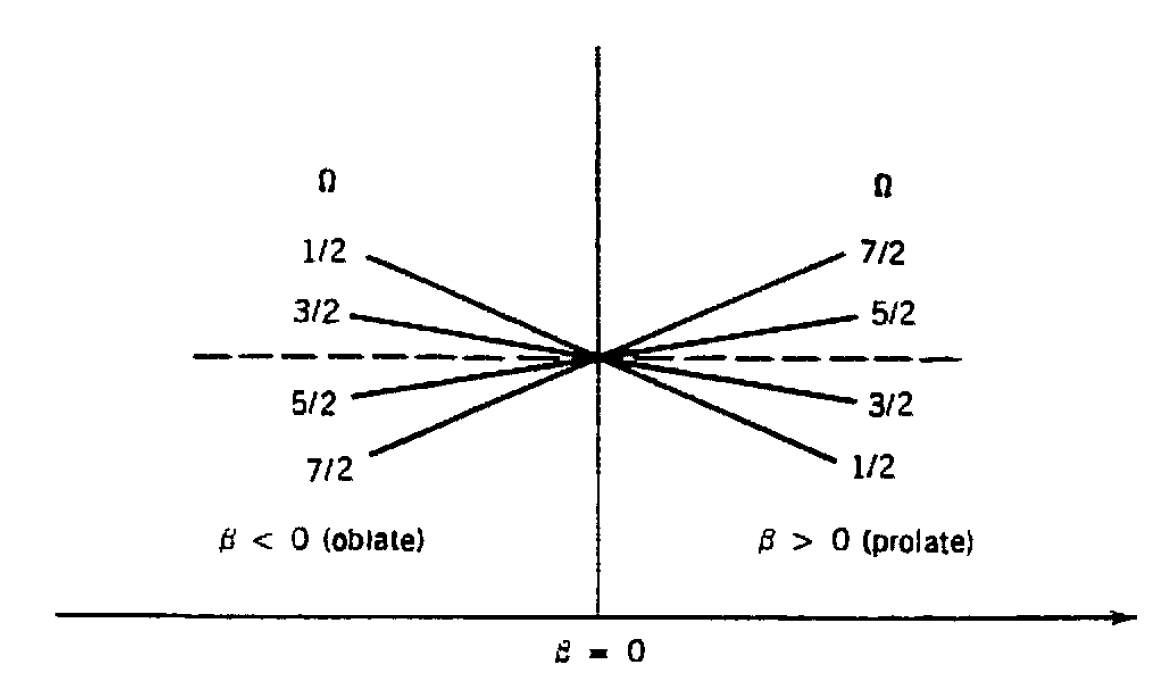
\includegraphics[scale=0.5]{images/levelsplit.png}
    \caption{Level splitting with deformation.~\cite[pg. 153]{krane}}
    \label{fig:levelsplit}
  \end{figure}
\item What does this have to do with fission? 
  \begin{enumerate}
  \item As the nucleus becomes more deformed ($\epsilon\uparrow$), if
    the nucleus is not stable under fission, its binding
    energy is going up like $\epsilon^2$ as it runs towards
    fission. The system total energy $E_T$ is going up with
    distortion. 
  \item Some valence nucleon energies go up and some go down (as discussed
    above). If the valence nucleons happen to be in a state above the
    dotted line (where their energy goes \textit{up} with
    deformation), they will add to $E_T$ as the nucleus gets more
    deformed and it goes up faster. Woohoo fission here we come.

  \item  This doesn't last forever. Eventually, as $E_T\uparrow$
    and it keeps getting more deformed, nucleons will start dropping
    into energy states where their energy goes \textit{down} with
    deformation. This happens because the \textit{real} diagram is super complicated and messy, (it's Figure 5.29 in Krane
    if you want to look at it). 
  \item Once enough of the valence electrons are in a state where
    their energy goes \textit{down} with deformation, they start
    driving the total energy $E_T$ down.
  \item Then you have to keep deforming until valence nucleons go to
    another state where their energy goes up with deformation.
  \item This makes a little valley of stability at the top of the
    energy vs. deformation diagram. This is shown in
    Figure~\ref{fig:fissionhumps}.~\cite[pp. 493-495]{krane}
  \end{enumerate}
  \begin{figure}[hbtp]
    \centering
    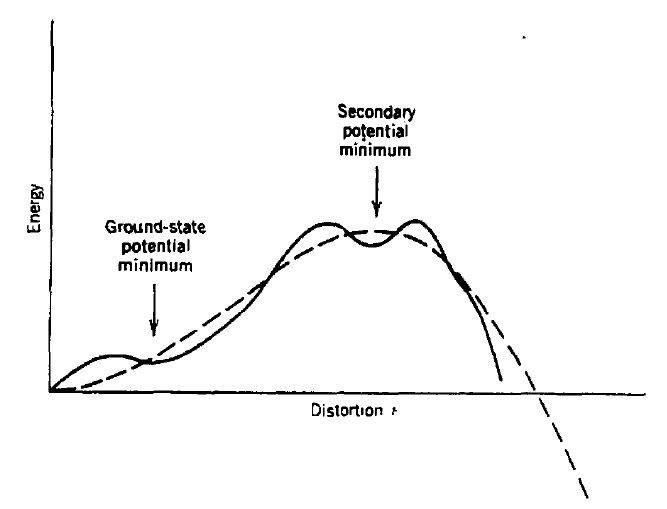
\includegraphics[scale=1.0]{images/shell_model}
    \caption{Energy with distortion. The solid line shows the change
      due to shell structure.~\cite[pp. 496]{krane}}
    \label{fig:fissionhumps}
  \end{figure}



\item This actually helps us cause fission, now we don't have to
  excite the nucleus all the way to the top of the barrier, we can
  just get to the bottom of that secondary well to make fission
  likely.~\cite[pp. 495]{krane}
\item The nucleus can hang out in this well. Just like any other
  potential well there are bound states with energy levels, this is
  called a \textit{fission isomer}. They generally have rotation bands
  (because they are deformed) and can either decay down to the
  ground state, or (usually) spontaneously fission. These are shape isomers,
  because the shape change required to go down to the ground state
  makes that transition much less likely.~\cite[pp. 495-496]{krane}
\end{itemize}

\subsection{Reactors}
\begin{itemize}
\item The neutron reproduction factor $k_\infty$ is the net change in
  thermal neutrons from one generation to the next. The $\infty$ is
  because we assume we're in an infinite reactor where no neutrons
  escape (leak). If $k_\infty$ = 1, we have the same number of neutrons
  each generation, the reactor is \textit{critical}. If $k_\infty
  > 1$, the reactor is \textit{supercritical} and if $k_\infty < 1$ the
  reactor is \textit{subcritical}.~\cite[pp. 501]{krane}
\item Fission events of \textsuperscript{235}U create approximately
  2.5 fast neutrons per fission. $\nu \approx$
  2.5.~\cite[pp. 501]{krane}
\item We know how many fast neutrons are made per fission, but not
  every thermal neutron absorbed causes fission. Sometimes it is just
  absorbed. To correct for this we use $\eta$:
  \begin{equation*}
    \eta = \nu\frac{\sigma_f}{\sigma_f+\sigma_a}
  \end{equation*}
Where $\sigma_f$ is the cross section for fission, and $\sigma_a$ is
the cross section for absorption that doesn't cause
fission.~\cite[pp.502]{krane}
\begin{framed}
  Note that the notation used by Krane is confusing. Fission is
  \textit{an absorption event}. Usually, \textbf{but not here}, the total absorption cross
  section $\sigma_a$ is defined as the sum of fission and other events
  (such as $\gamma$-decay): $\sigma_a = \sigma_f +
  \sigma_\gamma$. I'm going to stick with Krane's notation here. So
  remember, $\sigma_a$ is \textbf{absorption that doesn't cause
    fission} and does \textit{not} include $\sigma_f$.
\end{framed}
\item The
difference between $\eta$ and $\nu$ can be confusing:
\begin{itemize}
\item $\nu$: The number of fast neutrons per \textit{fission}.
\item $\eta$: The number of fast neutrons per \textit{thermal neutron
    absorbed} by fuel. This will always be lower than $\nu$ because
  some amount of neutrons will be absorbed and not cause fission
  ($\sigma_a$ above).
\end{itemize}
\item If we have $N$ thermal neutrons in the last generation that all get
  absorbed in our fuel, we will now have $N\eta$ new fast neutrons.
\item Rarely, these fast neutrons will actually cause fission (in
  \textsuperscript{238}U), which leads to a sliiiight increase in our
  total fast neutrons. We call this the \textit{fast fission factor}
  ($\epsilon$). It's usually small, like 1.03.~\cite[pp.502]{krane}
\item So now, we have $N\eta\epsilon$ fast neutrons.
\item The fission cross section is low for fast neutrons, so we want
  to reduce their energy (slow or moderate) them down to thermal
  energies where the fission cross section is high. Unfortunately, as
  they slow down, they have to go through the resonance region where
  there is a high probability of absorption that won't cause fission (by \textsuperscript{238}U
  for example). The probability that a
  given fast neutron manages to reach thermal without being absorbed
  is called the \textit{resonance escape probability}
  ($p$). Krane gives a value of 0.9.~\cite[pp. 503]{krane}
\item Now, of our $N\eta\epsilon$ fast neutrons, $N\eta\epsilon{}p$ have all slowed
  down to thermal energy.
\item Just because a neutron is thermal doesn't mean it will be
  absorbed in our fuel. Reactors are made up of a ton of steel and
  moderator (water or graphite), and other stuff. The neutrons might
  get absorbed in that instead of the fuel. So we use the
  \textit{thermal utilization factor} ($f$):
  \begin{equation*}
    f = \frac{\sigma_a^{\text{fuel}}+\sigma_f^{\text{fuel}}}{\sigma_a^{\text{all}}+\sigma_f^{\text{all}}}
  \end{equation*}
Where all means all the materials, including fuel. This is the
fraction of neutrons absorbed in the fuel instead of absorbed
somewhere else.~\cite[pp. 503]{krane}
\item Now, of our thermal neutrons, $N\eta\epsilon{}p$, we have
  $N\eta\epsilon{}pf$ that are actually absorbed in our fuel (remember
  we are talking about an infinite reactor, so they can't escape).
\item Finally, we can get $k_\infty$. Last generation we had $N$
  neutrons absorbed in our fuel, and now we have $N\eta\epsilon{}pf$
  neutrons in this generation absorbed in our fuel. $k_\infty$ is just
  the ratio of neutrons this generation to last generation:
  \begin{equation*}
    k_\infty = \frac{N\eta\epsilon{}pf}{N} = \eta\epsilon{}pf
  \end{equation*}
This is the \textit{four factor formula}.~\cite[pp. 503]{krane}
\item Effects that change one of the factors may affect the
  criticality of the reactor (by changing $k_\infty$).
  \begin{itemize}
  \item In a water-cooled reactor, if the temperature of the water
    goes up:
    \begin{itemize}
    \item Water is the moderator, it is used to slow down neutrons
      because hydrogen is great at removing neutron energy.
    \item As temperature goes up, water gets \textit{less} dense.
    \item Less dense water means collisions happen less frequently, so
      neutrons slow down slower and travel further.
    \item If it's harder to slow down to thermal energies, they spend
      more time in the resonance region, so there is a higher
      probability they will be resonantly absorbed.
    \item The resonance \textit{escape} probability goes
      \textit{down}, and overall $k_\infty$ goes down.
    \end{itemize}
  \end{itemize}
\end{itemize}
\section{Fusion \& Plasmas}

\subsection{Kinematics}
\begin{itemize}
\item The following fusion reaction:
  \begin{equation*}
    a + X \to Y + b
  \end{equation*}
will have product particles with energies that sum to the Q value of
the reaction:
\begin{equation*}
  \frac{1}{2}m_bv_b^2+\frac{1}{2}m_Yv^2_Y = Q
\end{equation*}
Which gives:
\begin{equation*}
  \frac{1}{2}m_bv^2_b = \frac{Q}{1+m_b/m_Y}
\end{equation*}
\begin{equation*}
  \frac{1}{2}m_Yv^2_Y = \frac{Q}{1+m_Y/m_b}
\end{equation*}
\cite[pp. 531]{krane}
\end{itemize}
\subsection{Energy}
\begin{itemize}
\item For the reaction to occur, the two reactants must have enough
  energy to overcome the Coulomb barrier given by:
  \begin{equation*}
    V_c = \frac{e^2}{4\pi\epsilon_0}\frac{Z_aZ_X}{R_a+R_X}
  \end{equation*}
You can generally assume each particle has half of this energy initially.
\item The rate of a nuclear reaction depends on the product of the
  cross section for the reaction to occur $\sigma$ and the speed of
  the particles $v$. Normally, for thermal neutron reactions outside the
  resonance region $\sigma \propto 1/v$, so $\sigma{}v$ is
  constant, this isn't true in fusion reactions.~\cite[pp. 532]{krane}
\item In thermonuclear fusion, at the high temperatures, the cross
  section $\sigma$ is not proportional to $1/v$, as seen in
  Figure~\ref{fig:fusion_xsec}. So $\sigma{}v$ will not be constant. The value of
  $\sigma{}v$ is averaged over all speeds and energies to get:
  $\braket{\sigma{}v}$.~\cite[pp. 533]{krane}
  \begin{figure}[hbtp]
    \centering
    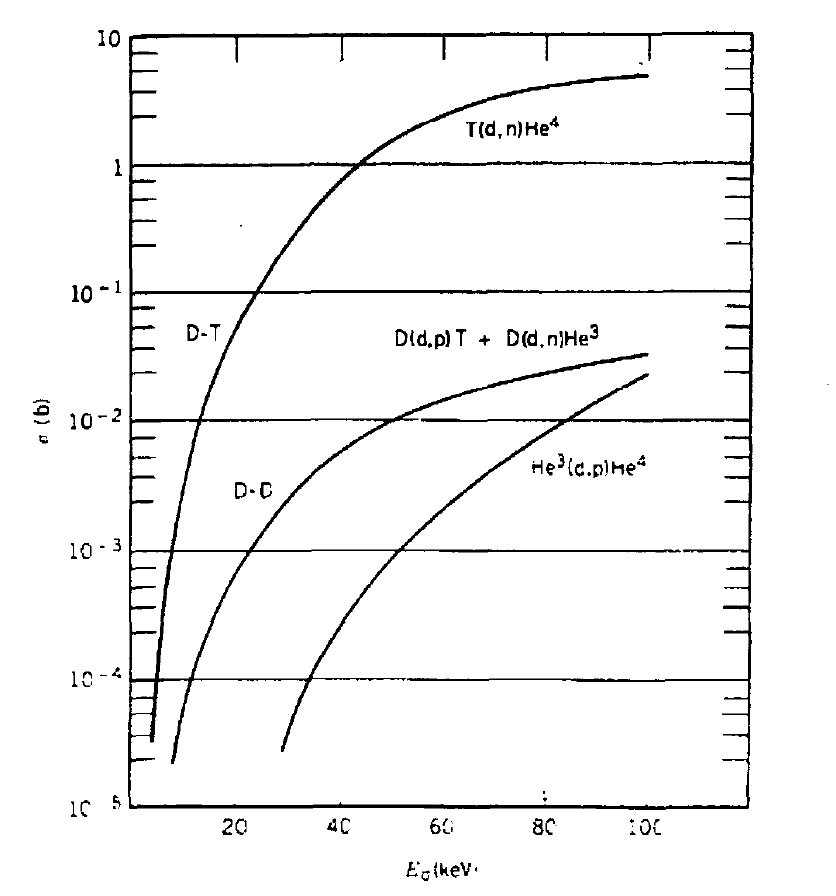
\includegraphics[scale=0.5]{images/fusion_xsection}
    \caption{Cross section for fusion
      reactions. $E_d$ is the energy of the deuteron in the fusion,
      which will be proportional to the speed of the particle.~\cite[pp. 532]{krane}}
    \label{fig:fusion_xsec}
  \end{figure}
\item The energy released in fusion is given by:
  \begin{equation*}
    E_f = \frac{1}{4}n^2\braket{\sigma\nu}Q\tau
  \end{equation*}
This assumes that we have $n$ density of particles causing fusion (like D
and T in a fuel pellet) and that there are equal amounts of both (the
individual densities are $\frac{1}{2}n$). $Q$ is the energy released
in the reaction, $\tau$ is the length of time the plasma is confined
and $\braket{\sigma{}v}$ is the average cross section times particle
velocity.~\cite[pp. 541]{krane}
\item The energy per unit volume required to heat the plasma is:
  \begin{equation*}
    E_{\text{th}} = 3nkT
  \end{equation*}
Where $n$ is the density of the particles, $k$ is the boltzman
constant and $T$ is the plasma temperature.~\cite[pp. 541]{krane}
\item Overall, if we heat the plasma using $E_{\text{th}}$ to a
  temperature $T$ and confine it at that temperature for time $\tau$,
  we get $E_f$ out. We have an overall net gain if $E_f >
  E_{\text{th}}$:
  \begin{equation*}
    \frac{1}{4}n^2\braket{\sigma{}v}Q\tau > 3nkT
  \end{equation*}
  \begin{equation*}
    n\tau > \frac{12kT}{\braket{\sigma{}v}Q}
  \end{equation*}
This $n\tau$ value is also called the ``Lawson criterion.''
\cite[pp. 541-542]{krane}
\item The $Q$ value for various parts of the fusion process can be
  defined:
  \begin{equation*}
    Q = \frac{P_{\text{out}}}{P_{\text{in}}} = \frac{E_{\text{out}}}{E_{\text{in}}}
  \end{equation*}
This can be used for multiple processes, including the reactor as a
whole. Note that for a reactor if they give you E$_{\text{thermal}}$,
it is the sum of the energy from the fusion \textit{and} the input energy.
\end{itemize}

\subsubsection{Losses}

\begin{itemize}
\item The primary way that a plasma loses energy is
  \textit{bremsstrahlung} (breaking radiation). When two particles Coulomb scatter in a
  plasma, they accelerate and release radiation. This is bad for our
  plasma because we want to keep as much of the energy in the
  particles as possible to keep them at a high enough energy to
  continue fusion.~\cite[pp. 539]{krane}
\item These bremsstrahlung losses are proportional to $Z^2$, so it is
  beneficial to use lighter nuclei (hydrogen and helium):
  \begin{equation*}
    P_{\text{br}}=0.5\times 10^{-36}Z^2n_{\text{ion}}n_e{(kT)}^{1/2}
  \end{equation*}
where P is in W/m$^3$, $n_{\text{ions}}$ and $n_e$ are the number
densities of the ions and electrons in the plasma, respectively, and $Z$ is the
charge of the ions. It's probably most important just to know that it's less
for lighter nuclei (due to $Z^2$), and that there is a temperature at which the gains
from fusion exceed the bremsstrahlung losses: 4 keV for D-T and 40 keV
for D-D.~\cite[pp. 540]{krane}
\item There are other losses, such as synchrotron radiation from the
  particles orbiting in the magnetic field, but these are negligible
  compared to the bremsstrahlung.~\cite[pp. 539]{krane}
\end{itemize}

\subsection{Plasma Reactions}
\begin{itemize}
\item Reaction rate is proportional to the speed of the particles, and
  the density of the particles.~\cite[Lec 28]{lecture}
\item In a thermal environment, the particles velocities have a
  Maxwell-Boltzmann distribution that is a function of
  temperature.~\cite[Lec 28]{lecture}
\item The Coulomb barrier makes reaction rates very low, all of the
  reaction rates drop to zero at low energy (this is true of all
  charged particle reactions) as seen in the upper portion of
  Figure~\ref{fig:charged_xsec}. We get through the coulomb barrier by
  tunneling.~\cite[Lec 28]{lecture}
  \begin{figure}[hbtp]
    \centering
    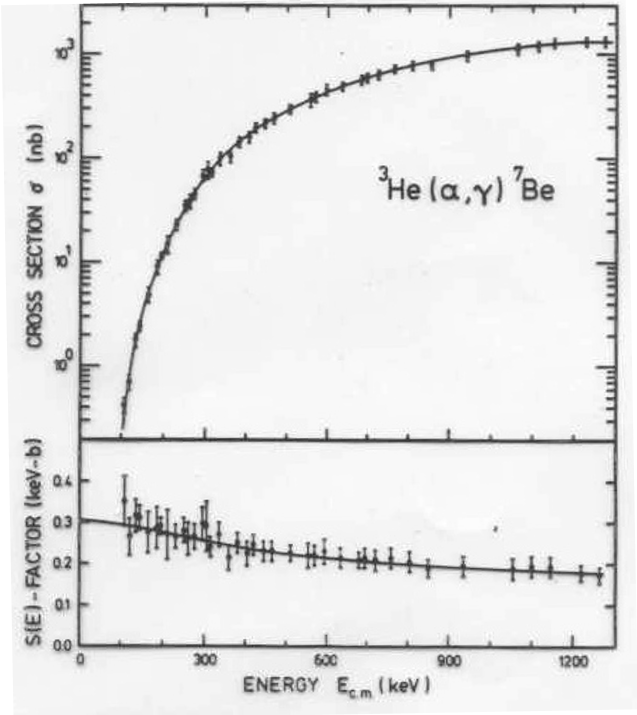
\includegraphics[scale=0.5]{images/charged_cross_section}
    \caption{Coulomb barrier for charged-particle induced
      reactions.~\cite[Lec. 28]{lecture}}
    \label{fig:charged_xsec}
  \end{figure}
\item All the cross sections look the same due to this Coulomb effect,
  so it would be beneficial to factor that out to see if anything else
  is going on. The $S(E)$ factor has the Coulomb effect removed, so
  you can see if there is an impact on the cross section from
  \textit{nuclear} effects. This is seen in the lower part of
  Figure~\ref{fig:charged_xsec}. The slight rise shows that there is
  some broad resonance at low energies in this reaction, there must be
  an accessible energy state at low energies that favors this
  reaction.~\cite[Lec. 28]{lecture}
\item The $S$-factor explains why the D+T reaction is so favored over
  the p+p reaction. They both have the \textit{same} Coulomb repulsion
  and the same thermal distribution
  that affects the rate, it's the $S$-factors are what is
  different. In this case, it's because p+p is weak force mediated,
  D+T is a strong force reaction.~\cite[Lec. 28]{lecture}
\item In the region between the exponential probability of tunneling
  and the Maxwell-Boltzman thermal distribution, there is a window
  where the reaction can actually occur. This is called the Gamow peak
  (Coulomb barrier and thermal distribution together, assumes
  $S$-factor has no effect).~\cite[Lec. 28]{lecture}
\item The effective Coulomb barrier can be reduced by the electron
  cloud, which ``screen'' the positive charge of the nucleus and allow
  other charged particles to get closer before repulsion
  occurs.~\cite[Lec 28]{lecture}
\end{itemize}

\subsection{NIF}
\begin{itemize}
\item There are 3 steps: Compress the capsule, the ``hot spot''
  ignites and the $\alpha$-particles cause runaway burn in the
  surrounding cold shell.~\cite[Lec. 29]{lecture}
\item We are relying on the $\alpha$-particles to heat the plasma and
  keep the reaction going. The released 14 MeV neutrons are what we
  are interested in using for power, they leave a lot of their energy
  behind in scattering before getting out of the
  plasma.~\cite[Lec. 29]{lecture}
\item Due to the fact that we use $\alpha$-particles to heat the
  plasma, we define the $Q_\alpha$ parameter:
  \begin{equation*}
    Q_\alpha = \left(\frac{E_\alpha}{E^{\text{thermal}}_{\text{input}}}\right)
  \end{equation*}
Which is just the ratio of energy returned from the $\alpha$-particles
to the plasma, divided by the energy put into the plasma. Some values
are shown in Table~\ref{tab:q-alpha}.
\begin{table}[hbtp]
\centering
\begin{tabular}{ll}
$Q_\alpha$ &  Status\\
2 & $\alpha$-heating \\
10 & $\alpha$-dominated plasma ``burning plasma'' \\
400 & theoretically possible at NIF
\end{tabular}
\caption{$Q_\alpha$ values for NIF.~\cite[Lec. 29]{lecture}}
\label{tab:q-alpha}
\end{table}
\end{itemize}

\section{Detectors}
\begin{itemize}
\item Two modes: pulse mode: radiation are well-separated in time,
  current mode: radiation overlap at the detector
  location, they all pile up and you can't tell the radiation apart.~\cite[Lec. 36]{lecture}
\item Can measure any kind of ionization producing radiation,
  $\alpha$, $\beta$, $\gamma$, $p$, $d$, $t$, etc. They interact and
  deposit energy in the detector via the electromagnetic
  force. Neutrons are detected through their interactions with other
  matter, so you need a lot of matter.~\cite[Lec. 36]{lecture}
\item Feather's Rule: A rule of thumb for the range of an electron (in
  g/cm$^2$) is:
  \begin{equation*}
    R = \frac{E_{max} \text{MeV}}{2}
  \end{equation*}
The range is an areal density (in g/cm$^2$), so you can divide by
density to get a thickness.~\cite[Lec. 36]{lecture}
\item Stopping power identifies the rate of energy loss of the ion in
  a material. This is given by the Bethe-Bloch formula that is ugly
  and not even worth typing out here. You can solve for the range that
  the particle will go:
  \begin{equation*}
    R = \int^0_T{\left(\frac{-dE}{dx}\right)}^{-1}dE
  \end{equation*}
Where $dE/dx$ is that Bethe-Bloch formula. I guess this would be
useful if he gives you that and asks how far a particle will go.~\cite[Lec. 36]{lecture}
\item Ions interact with electrons, the majority of the stopping is
  due to these electronic interactions. This is dominated by the fact
  that there are so many electrons in so many large areas (atoms are
  huge compared to nuclei) so the probability of interacting with
  electrons is \textit{much} higher than nuclei.~\cite[Lec. 36]{lecture}
\end{itemize}
\subsection{Types}
\begin{itemize}
\item Gas-filled detectors: incoming radiation creates electron-ion
  pairs and the current is detected.~\cite[Lec.36]{lecture}
\item Photomultiplier tubs (PMT): An incoming photon interacts with a
  photo-cathode, releasing an electron. This electron travels through
  a series of dynodes that create more and more electrons in a
  cascade (hence, multiplier). This is
  measured.~\cite[Lec. 36]{lecture}
\item Scintillation detector: incoming light releases loosely bound
  photoelectrons. These are generally coupled to photomultiplier tubes.
\end{itemize}

\bibliographystyle{unsrt}
\bibliography{../NE101}
\end{document}
